\documentclass{standalone}
\usepackage{graphicx}	
\usepackage{amssymb, amsmath, amsthm}
\usepackage{color}

\usepackage{tikz}
\usetikzlibrary{intersections, backgrounds}

\definecolor{light}{RGB}{220, 188, 188}
\definecolor{mid}{RGB}{185, 124, 124}
\definecolor{dark}{RGB}{143, 39, 39}
\definecolor{highlight}{RGB}{180, 31, 180}
\definecolor{gray10}{gray}{0.1}
\definecolor{gray20}{gray}{0.2}
\definecolor{gray30}{gray}{0.3}
\definecolor{gray40}{gray}{0.4}
\definecolor{gray60}{gray}{0.6}
\definecolor{gray70}{gray}{0.7}
\definecolor{gray80}{gray}{0.8}
\definecolor{gray90}{gray}{0.9}
\definecolor{gray60}{gray}{0.95}

\begin{document}

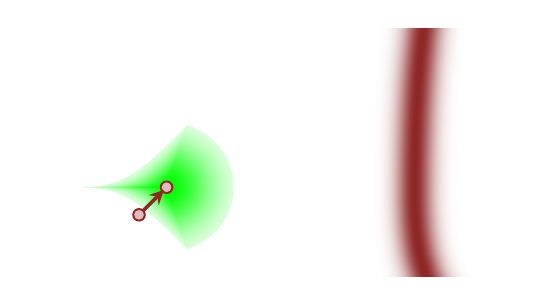
\begin{tikzpicture}[scale=0.35, thick]
  \draw[white] (-6, -3) rectangle (12, 6);
  
  \pgfmathsetmacro{\x}{-1}
  \pgfmathsetmacro{\y}{0.25}
  \pgfmathsetmacro{\delta}{3}
  \foreach \i in {1, 0.99, ..., 0} {
    \pgfmathsetmacro{\prop}{100 * exp(-2.0 * \i * \i)};
    \colorlet{custom}{green!\prop!white};
    \fill[custom]
      ({\x - \delta * \i}, \y) 
      .. controls ({\x - 0.5 * \delta * \i}, \y) 
        and ({\x - 0.25 * \delta * \i}, {\y - 0.25 * \delta * \i}) 
      .. ({\x + 0.25 * \delta * \i}, {\y - 0.75 * \delta * \i})
      .. controls ({\x + \delta * \i}, {\y - 0.5 * \delta * \i}) 
         and ({\x + \delta * \i}, {\y + 0.5 * \delta * \i}) 
       .. ({\x + 0.25 * \delta * \i}, {\y + 0.75 * \delta * \i})
       .. controls ({\x - 0.25 * \delta * \i}, {\y + 0.25 * \delta * \i}) 
         and ({\x - 0.5 * \delta * \i}, \y) .. ({\x - \delta * \i}, \y);
  }
  \fill[color=dark] (-1, 0.25) circle (7pt); 
  \fill[color=light] (-1, 0.25) circle (5pt);

  \draw[color=dark, ->, >=stealth, line width=1.25] (-2, -0.75) -- +(0.9 * 1, 0.9 * 1);

  \fill[color=dark] (-2, -0.75) circle (7pt); 
  \fill[color=light] (-2, -0.75) circle (5pt);

  \begin{scope}
    \clip (-6, -3) rectangle (12, 6);
  \foreach \i in {1, 0.99, ..., 0} {
    \pgfmathsetmacro{\prop}{100 * exp(-5.0 * \i * \i)};
    \colorlet{custom}{dark!\prop!white};
      \draw[line width={30 * \i}, color=custom] 
        (8, 0) .. controls (8, 1.5 * 15) and (18,  1.5 * 5) .. (18,  1.5 * 5)
        .. controls (23,  1.5 * 5) and (28,  1.5 * 8) .. (28, 0)
        .. controls (28, - 1.5 * 8) and (23, - 1.5 * 3) .. (18, - 1.5 * 3)
        .. controls (13, - 1.5 * 3) and (8, - 1.5 * 5) .. (8, 0);
    }  
  \end{scope}

\end{tikzpicture}

\end{document}  